\documentclass{beamer}
\usepackage[utf8]{inputenc}
\usepackage{graphicx}
\usepackage{hyperref}

% Tema base
\usetheme{Madrid}

% Pie de página con autores, título del tema y número de slide
\setbeamertemplate{footline}{
  \leavevmode%
  \hbox{
    \begin{beamercolorbox}[wd=.3\paperwidth,ht=2.5ex,dp=1.5ex,left]{author in head/foot}
      \usebeamerfont{author in head/foot}Edgar Ivan Calpa (UNAL Manizales)
    \end{beamercolorbox}
    \begin{beamercolorbox}[wd=.349\paperwidth,ht=2.5ex,dp=1.5ex,center]{title in head/foot}
      \usebeamerfont{title in head/foot} EEGNet y Shallow ConvNet
    \end{beamercolorbox}
    \begin{beamercolorbox}[wd=.328\paperwidth,ht=2.5ex,dp=1.5ex,center]{date in head/foot}
    \hspace*{-0.5cm} % mueve el texto hacia la izquierda
    \usebeamerfont{date in head/foot}                 \insertframenumber/\inserttotalframenumber
    \end{beamercolorbox}
  }
  \vskip0pt%
}

% Datos de la presentación
\title{EEGNet y Shallow ConvNet}
\author[Edgar Ivan Calpa Cuacialpud]{Universidad Nacional de Colombia - Sede Manizales \\\\ Edgar Ivan Calpa Cuacialpud \small }
\date{Modelos de aprendizaje profundo aplicados a señales EEG: EEGNet y Shallow ConvNet\\ 
Profesor: Andrés Marino Álvarez Meza, PhD\\ 
Departamento de ingeniería eléctrica, electrónica y computación }


\setbeamertemplate{caption}[numbered]

% En el preámbulo de tu documento
\usepackage{hyperref} % para enlaces clicables


\begin{document}

% Diapositiva de título con logo
\begin{frame}
    \titlepage
    \vspace{0cm} % sube el logo (ajusta el valor)
    \begin{center}
        
\includegraphics[width=0.3\linewidth]{UNM.png}
    \end{center}
\end{frame}


% Introducción
\begin{frame}{Introducción}
\begin{columns}[T]

    % Columna izquierda: texto
    \begin{column}{0.55\textwidth}
Este esquema muestra un enfoque multimodal para el reconocimiento de emociones que combina señales EEG y análisis de video facial.  
Incluye la construcción de redes cerebrales en distintos dominios (frecuencia, tiempo y wavelet), extracción de características relevantes y su fusión para la clasificación final.
    \end{column}

    % Columna derecha: imagen con enlace y referencia
    \begin{column}{0.48\textwidth}
        \begin{figure}
            \centering
            \href{https://www.nature.com/articles/s41598-025-98404-2/figures/1}{%
                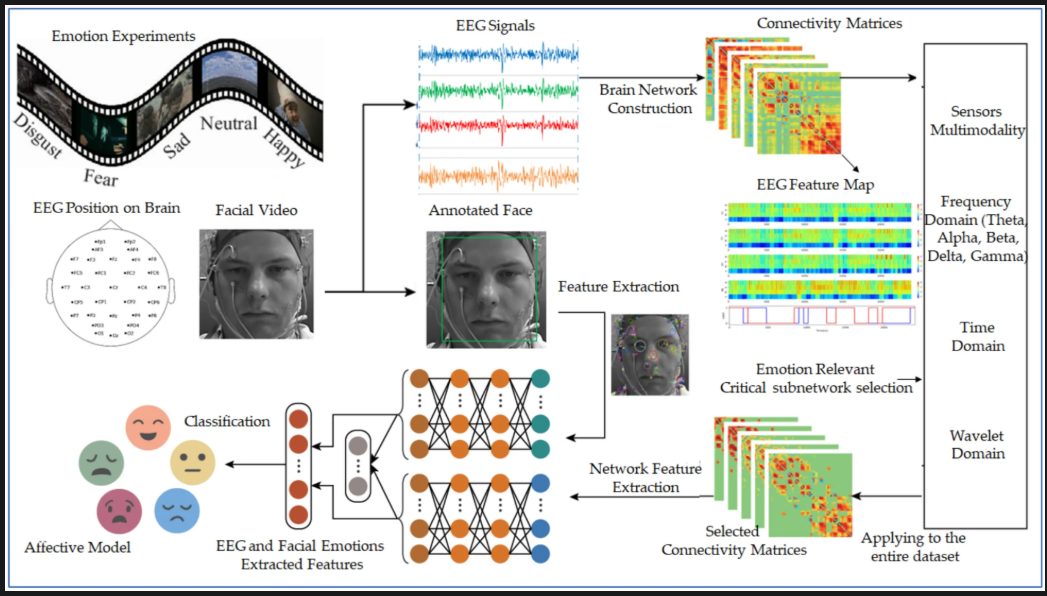
\includegraphics[width=\linewidth]{figura_emotrans.png}%
            }
            \caption{\small Pipeline multimodal EEG–video para clasificación de emociones.}
            \label{fig:multimodal_emotion}
        \end{figure}
    \end{column}

\end{columns}
\end{frame}


% Introducción
\begin{frame}{Introducción}
\begin{columns}[T] % [T] alinea el contenido arriba

    % Columna izquierda: texto
    \begin{column}{0.55\textwidth}
Ante estas limitaciones, han surgido arquitecturas de aprendizaje profundo diseñadas específicamente para abordar la complejidad de las señales EEG.  
En esta revisión se analizan dos modelos representativos:  
\textbf{EEGNet}, una arquitectura compacta basada en convoluciones separables que busca eficiencia y generalización; y  
\textbf{Shallow ConvNet}, una red convolucional superficial orientada a la extracción de ritmos mu y beta en tareas de imaginación motora.
    \end{column}

    % Columna derecha: imagen con enlace y referencia
    \begin{column}{0.4\textwidth}
        \begin{figure}
            \centering
            \href{https://www.mdpi.com/1424-8220/22/21/8250}{%
                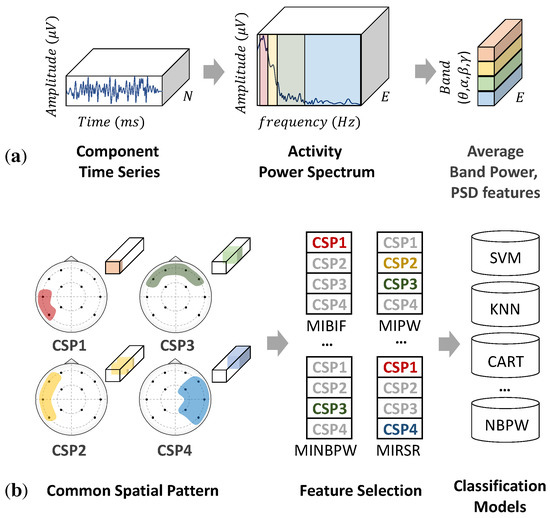
\includegraphics[width=\linewidth]{sensors-22-08250-g001-550.jpg}%
            }
            \caption{\small Pipeline de procesamiento y clasificación de EEG con métodos tradicionales y redes convolucionales.}
            \label{fig:eeg_models}
        \end{figure}
    \end{column}

\end{columns}
\end{frame}



% Introducción
\begin{frame}{Introducción: Enfoque clásico vs. aprendizaje profundo}
\scriptsize
\begin{table}[h]
\centering
\renewcommand{\arraystretch}{1.3}
\begin{tabular}{|p{2cm}|p{4cm}|p{4cm}|}
\hline
\textbf{Etapa} & \textbf{Enfoque clásico} & \textbf{Aprendizaje profundo (EEGNet / Shallow ConvNet)} \\
\hline
Entrada & Señal EEG preprocesada (filtrada, segmentada) & Señal EEG cruda o mínimamente preprocesada \\
\hline
Extracción de características & Manual: PSD, potencia por banda, CSP & Automática: convoluciones aprenden patrones espaciales y temporales \\
\hline
Selección de características & MIBIF, MIPW, PCA, LDA & No se requiere: la red aprende qué es relevante \\
\hline
Modelos de clasificación & SVM, KNN, CART, Naive Bayes & Redes neuronales convolucionales (CNN) \\
\hline
Ventajas & Interpretabilidad, bajo costo computacional & Generalización, robustez, menos ingeniería manual \\
\hline
Limitaciones & Dependencia de expertos, sensibilidad al ruido & Requiere más datos y entrenamiento computacional \\
\hline
\end{tabular}
\caption{Comparación entre el enfoque clásico y el enfoque basado en aprendizaje profundo para clasificación de señales EEG.}
\end{table}
\end{frame}



% Introducción
\begin{frame}{Introducción}

El objetivo de esta revisión es identificar los problemas específicos que cada modelo intenta resolver, analizar sus enfoques técnicos y evaluar su desempeño experimental en tareas de clasificación EEG. Esta base teórica servirá como fundamento para la fase experimental del trabajo de grado, en la cual se implementarán y compararán ambos modelos sobre conjuntos de datos públicos, documentando los resultados en un repositorio reproducible.

\begin{figure}[h]
    \centering
    \href{https://www.mdpi.com/1424-8220/22/21/8250}{%
        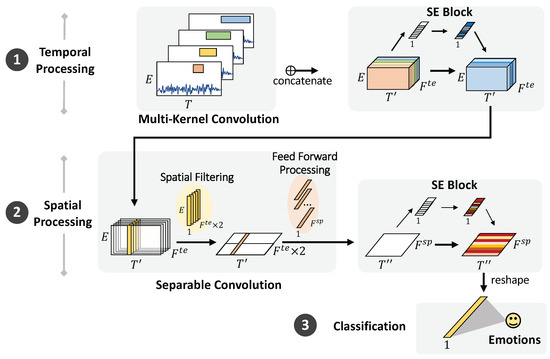
\includegraphics[width=0.43\linewidth]{temporalprocessing.jpg}%
    }
    \caption{\small Arquitectura de red neuronal para clasificación de emociones basada en EEG con procesamiento temporal y espacial.}
    \label{fig:eeg_models}
\end{figure}

\end{frame}

% EEGNet – Introducción
\begin{frame}{EEGNet – Introducción}
\begin{columns}[T] % [T] alinea arriba

    % Columna izquierda: texto
    \begin{column}{0.55\textwidth}
        \begin{block}{Contexto}
            EEGNet es una arquitectura de red neuronal convolucional compacta 
            diseñada para la clasificación de señales EEG en interfaces 
            cerebro-computador (BCI). Su desarrollo responde a la necesidad de 
            modelos capaces de manejar la alta variabilidad, el bajo nivel de 
            señal y la naturaleza no estacionaria del EEG, factores que dificultan 
            la generalización entre sujetos y paradigmas.
        \end{block}
    \end{column}

    % Columna derecha: imagen con enlace y referencia
    \begin{column}{0.45\textwidth}
        \begin{figure}
            \centering
            % El enlace envuelve solo la imagen
            \href{https://www.nature.com/articles/s41598-025-00824-7/figures/1}{%
                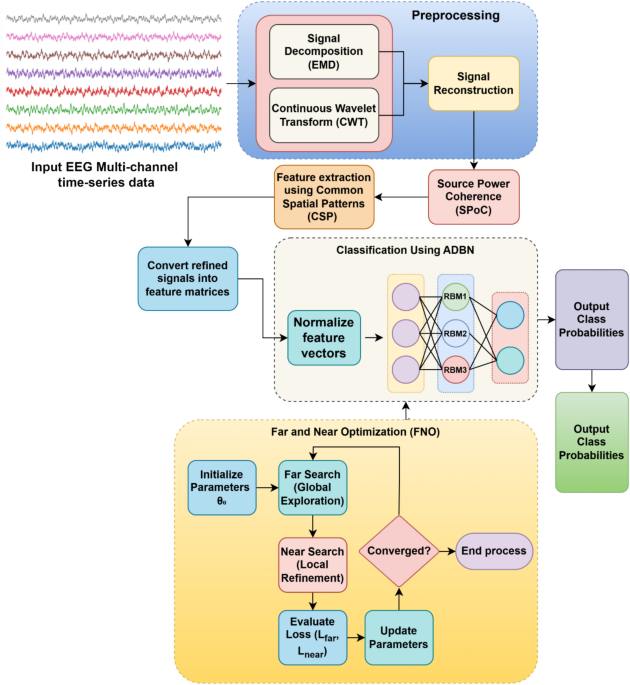
\includegraphics[width=\linewidth]{motorimageryEEG.png}%
            }
            \caption{\small Flujo de procesamiento del modelo propuesto para clasificación de EEG de imaginación motora. Adaptado de \textcite{Mathiyazhagan2025MI}.}
            \label{fig:flujo_eeg}
        \end{figure}
    \end{column}

\end{columns}
\end{frame}


% EEGNet – Introducción
% Activa numeración de figuras en Beamer (poner en el preámbulo si quieres numerar)
\begin{frame}{EEGNet – Introducción}
\begin{columns}[T] % [T] alinea arriba
    % Columna izquierda: texto
    \begin{column}{0.55\textwidth}
        \begin{block}{Problema que aborda}
En el procesamiento de EEG, los métodos tradicionales requieren ingeniería manual de características y suelen estar optimizados para un único paradigma BCI, lo que limita su aplicabilidad. EEGNet busca superar estas limitaciones ofreciendo un diseño versátil que pueda adaptarse a múltiples paradigmas como P300, ERN, MRCP y SMR.
        \end{block}
    \end{column}

    % Columna derecha: imagen con figura numerada y enlace
    \begin{column}{0.4\textwidth}
        \begin{figure}
            \centering
            \href{https://www.nature.com/articles/s41598-018-31673-2/figures/2}{%
                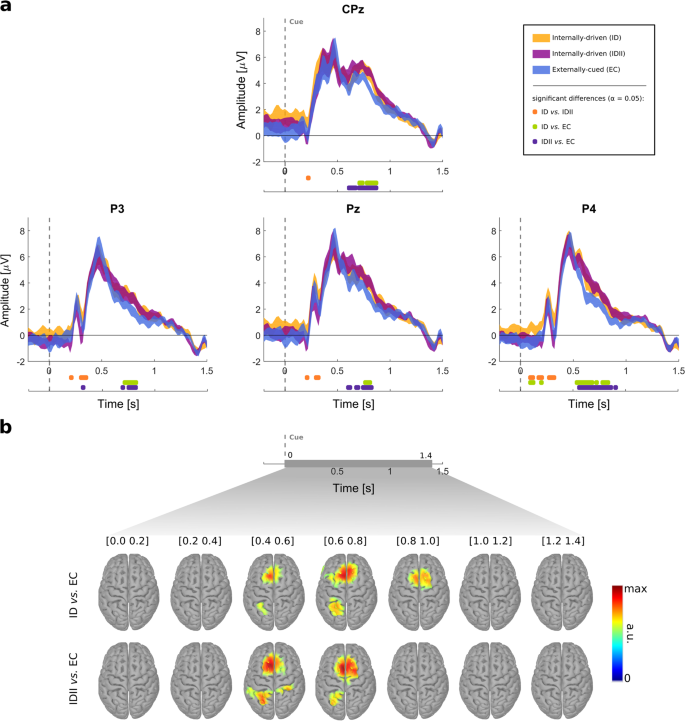
\includegraphics[width=\linewidth]{EEGpatterns.png}%
            }
            \caption{\small Comparación de ERPs y mapas de actividad cerebral entre condiciones de control interno y externo}
            \label{fig:flujo_eeg}
        \end{figure}
    \end{column}
\end{columns}
\end{frame}


% EEGNet – Introducción
% Activa numeración de figuras en Beamer (poner en el preámbulo)
\begin{frame}{EEGNet – Introducción}
\begin{columns}[T] % [T] alinea arriba
    % Columna izquierda: texto
    \begin{column}{0.45\textwidth}
\begin{block}{Motivación del diseño}
EEGNet emplea convoluciones separables (depthwise y pointwise) para extraer de forma eficiente características temporales y espaciales, junto con normalización por lotes y dropout para mejorar la generalización. Su bajo número de parámetros lo hace ideal para trabajar con conjuntos de datos limitados y para aplicaciones en tiempo real.
        \end{block}
    \end{column}

    % Columna derecha: imagen con figura numerada
    \begin{column}{0.55\textwidth}
        \begin{figure}
            \centering
            \href{https://www.mdpi.com/2227-7390/12/20/3286}{%
            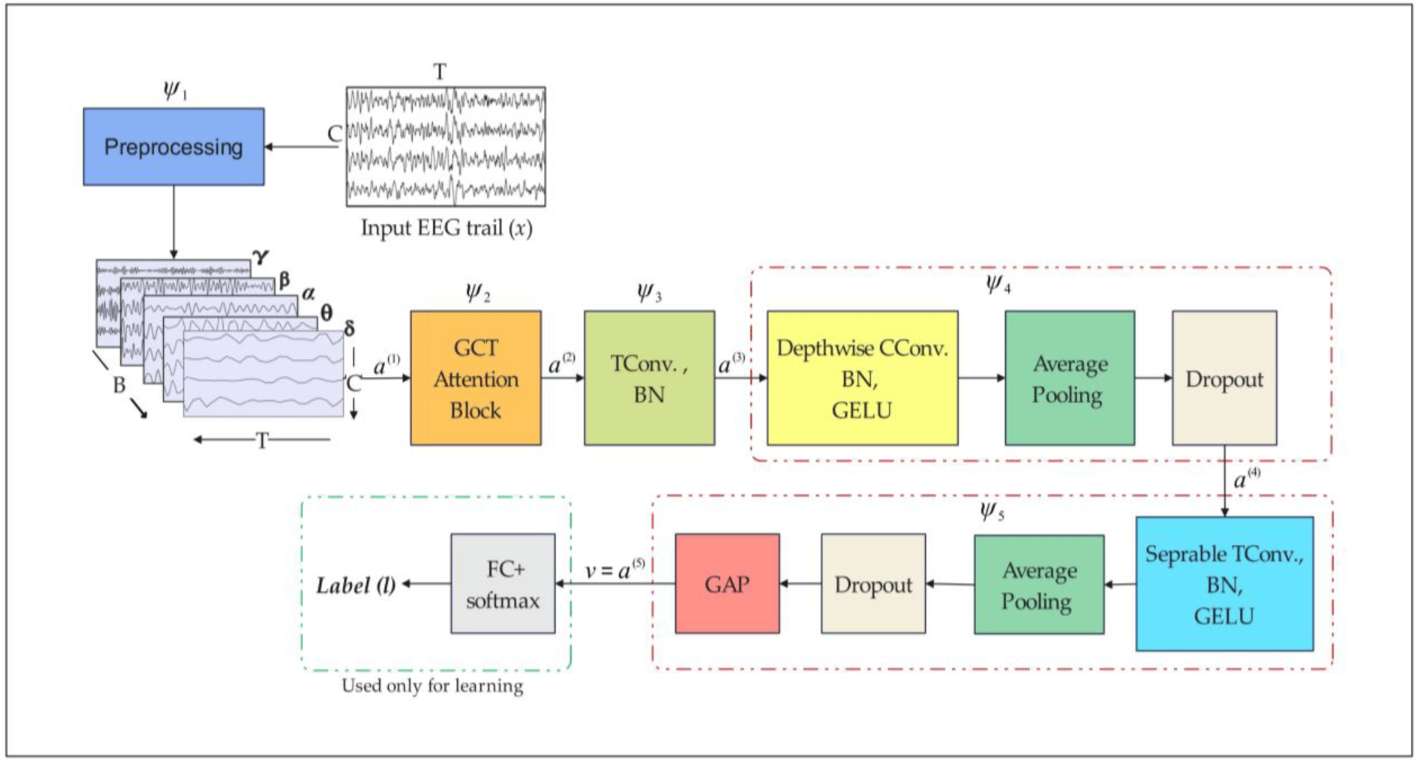
\includegraphics[width=\linewidth]{lightweight.png}%
            }
            \caption{\small Arquitectura del modelo GCT–EEGNet para reconocimiento de individuos basado en EEG}
            \label{fig:flujo_eeg}
        \end{figure}
    \end{column}
\end{columns}
\end{frame}

% EEGNet – Experimentos
\begin{frame}{EEGNet – Experimentos}
\begin{columns}[T] % [T] alinea arriba
    % Columna izquierda: texto
    \begin{column}{0.50\textwidth}
\begin{block}{Experimentos}
Los autores evaluaron EEGNet en cuatro paradigmas BCI: P300, ERN, MRCP y SMR. Se realizaron pruebas tanto intra-sujeto como entre sujetos, comparando el rendimiento de EEGNet con otros modelos convolucionales estándar.    

Los datasets utilizados incluyen registros públicos de EEG con tareas de imaginación motora y estímulos visuales. Las métricas principales fueron precisión (accuracy), coeficiente kappa y área bajo la curva (AUC), dependiendo del paradigma.
        \end{block}
    \end{column}

    % Columna derecha: imagen con figura numerada
    \begin{column}{0.5\textwidth}
        \begin{figure}
            \centering
            \href{https://ar5iv.labs.arxiv.org/html/1611.08024}{%
            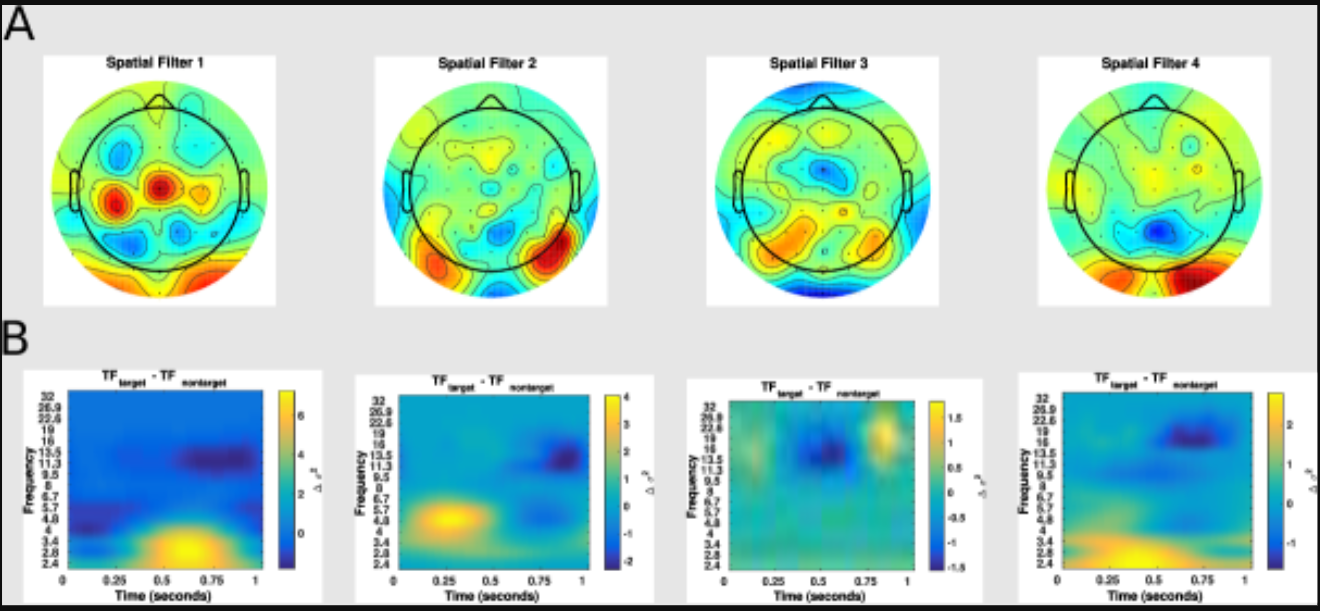
\includegraphics[width=\linewidth]{compactConvolutional.png}%
            }
            \caption{\small Filtros espaciales y representaciones tiempo‑frecuencia aprendidas por EEGNet}
            \label{fig:flujo_eeg}
        \end{figure}
    \end{column}
\end{columns}
\end{frame}

% EEGNet – Experimentos
\begin{frame}{EEGNet – Experimentos}
\begin{columns}[T] % [T] alinea arriba
    % Columna izquierda: texto
    \begin{column}{0.50\textwidth}
\begin{block}{Experimentos}

Los resultados mostraron que EEGNet supera a modelos más grandes en escenarios con datos limitados, especialmente en tareas de clasificación entre sujetos. En el paradigma ERN, por ejemplo, EEGNet obtuvo resultados significativamente superiores (p < 0.05) frente a otras CNN. Además, demostró ser robusto frente a ruido y variabilidad inter-sujeto, lo que lo convierte en una opción viable para aplicaciones clínicas y experimentales.
        \end{block}
    \end{column}

    % Columna derecha: imagen con figura numerada
    \begin{column}{0.5\textwidth}
        \begin{figure}
            \centering
            \href{https://ar5iv.labs.arxiv.org/html/1611.08024}{%
            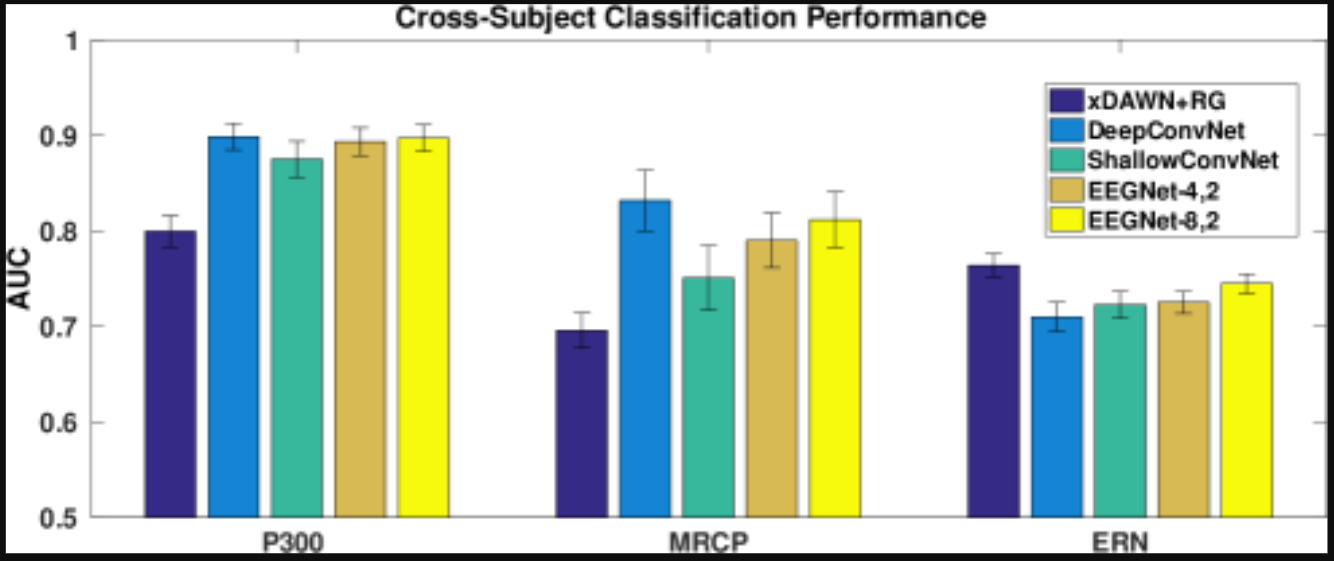
\includegraphics[width=\linewidth]{EEGNet.png}%
            }
            \caption{\small Rendimiento en clasificación entre sujetos (AUC) para P300, MRCP y ERN”}
            \label{fig:flujo_eeg}
        \end{figure}
    \end{column}
\end{columns}
\end{frame}

% EEGNet – Experimentos
\begin{frame}{EEGNet – Experimentos}
\begin{columns}[T] % [T] alinea arriba
    % Columna izquierda: texto
    \begin{column}{0.50\textwidth}
\begin{block}{Experimentos}

Entre las limitaciones observadas se encuentra la sensibilidad a la configuración de preprocesamiento y la necesidad de ajustar hiperparámetros según el paradigma específico. No obstante, su bajo costo computacional y versatilidad lo posicionan como un modelo base ideal para estudios comparativos en BCI.
        \end{block}
    \end{column}

    % Columna derecha: imagen con figura numerada
    \begin{column}{0.5\textwidth}
        \begin{figure}
            \centering
            \href{https://www.sciencedirect.com/science/article/pii/S0893608024007718}{%
            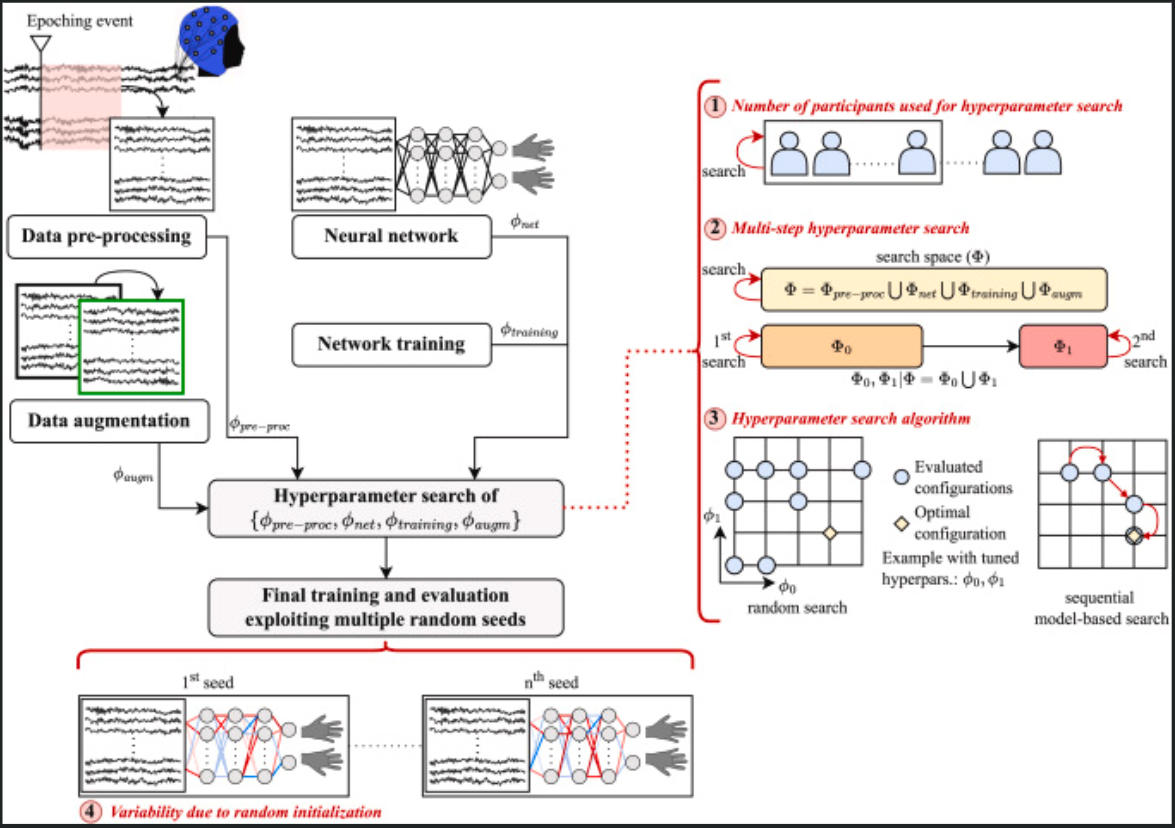
\includegraphics[width=\linewidth]{EEGdecoding.png}%
            }
            \caption{\small Esquema del protocolo de decodificación propuesto y de los experimentos realizados (marcados en rojo).}
            \label{fig:flujo_eeg}
        \end{figure}
    \end{column}
\end{columns}
\end{frame}

% Shallow ConvNet – Introducción
\begin{frame}{Shallow ConvNet – Introducción}
\begin{block}{Contexto}
Shallow ConvNet es una arquitectura convolucional diseñada para la clasificación de señales EEG, especialmente en tareas de imaginación motora (Motor Imagery). Su enfoque se centra en la extracción de ritmos mu y beta, que están directamente relacionados con la actividad motora cortical.
\end{block}
\end{frame}

% Shallow ConvNet – Introducción
\begin{frame}{Shallow ConvNet – Introducción}
\begin{block}{Problema que aborda}
Las señales EEG presentan alta variabilidad entre sujetos, ruido fisiológico y baja relación señal/ruido. Además, los métodos tradicionales requieren ingeniería manual de características, lo que limita la escalabilidad y reproducibilidad de los sistemas BCI.
\end{block}
\end{frame}

% Shallow ConvNet – Introducción
\begin{frame}{Shallow ConvNet – Introducción}
\begin{block}{Motivación del diseño}
La arquitectura de Shallow ConvNet combina convoluciones temporales para capturar la dinámica de la señal y convoluciones espaciales para modelar la distribución entre electrodos. Su diseño simple y reproducible lo convierte en un baseline ideal para estudios comparativos y benchmarking en bibliotecas como Braindecode.
\end{block}
\end{frame}


% Shallow ConvNet – Experimentos
\begin{frame}{Shallow ConvNet – Experimentos}
\begin{block}{Experimentos}
Shallow ConvNet fue evaluado principalmente en tareas de imaginación motora (Motor Imagery) utilizando el dataset BCI Competition IV 2a. El modelo se diseñó para extraer características espectrales y temporales asociadas a los ritmos mu y beta, relevantes en la actividad motora cortical.

La arquitectura combina convoluciones temporales para capturar la dinámica de la señal EEG y convoluciones espaciales para modelar la distribución entre electrodos. Se aplicaron pruebas intra-sujeto y entre sujetos, comparando su rendimiento con modelos más profundos y variantes de CNN.
\end{block}
\end{frame}

% Shallow ConvNet – Experimentos
\begin{frame}{Shallow ConvNet – Experimentos}
\begin{block}{Experimentos}
Los resultados mostraron que Shallow ConvNet logra una alta precisión en tareas de clasificación de imaginación motora, con métricas como accuracy y F1-score superiores a modelos más complejos en ciertos escenarios. En el dataset BCI IV 2a, alcanzó una precisión promedio superior al 80% en sujetos con señales limpias.

Su rendimiento se mantuvo estable incluso con configuraciones de preprocesamiento mínimas, lo que lo hace atractivo para implementaciones rápidas y entornos con recursos limitados.
\end{block}
\end{frame}

% Shallow ConvNet – Experimentos
\begin{frame}{Shallow ConvNet – Experimentos}
\begin{block}{Experimentos}
Entre las limitaciones observadas se encuentra su sensibilidad a artefactos musculares y oculares, así como una menor capacidad de generalización entre sujetos sin ajustes específicos. Además, su arquitectura fija requiere adaptación manual para distintos paradigmas BCI.

A pesar de ello, Shallow ConvNet se considera un baseline robusto y reproducible para estudios comparativos, y ha sido ampliamente adoptado en bibliotecas como Braindecode para benchmarking de modelos EEG.
\end{block}
\end{frame}


% Discusión Comparativa – Problema que resuelven
\begin{frame}{Discusión Comparativa – Problema que resuelven}
\begin{block}{Comparación}
\textbf{EEGNet} está diseñado para abordar la alta variabilidad, el bajo nivel de señal y la naturaleza no estacionaria de las señales EEG, ofreciendo una arquitectura versátil capaz de adaptarse a múltiples paradigmas BCI (P300, ERN, MRCP, SMR).  

\textbf{Shallow ConvNet}, por su parte, se enfoca en la extracción eficiente de características espectrales y temporales asociadas a ritmos mu y beta, optimizando su rendimiento en tareas de imaginación motora (Motor Imagery).
\end{block}
\end{frame}

% Discusión Comparativa – Complejidad computacional
\begin{frame}{Discusión Comparativa – Complejidad computacional}
\begin{block}{Comparación}
\textbf{EEGNet} emplea convoluciones separables y un número reducido de parámetros, lo que le otorga un bajo costo computacional y lo hace apto para aplicaciones en tiempo real y dispositivos con recursos limitados.  

\textbf{Shallow ConvNet} presenta una arquitectura más simple y menos profunda, lo que facilita su entrenamiento y reproducibilidad, aunque su diseño fijo puede requerir ajustes manuales para otros paradigmas.
\end{block}
\end{frame}

% Discusión Comparativa – Precisión y generalización
\begin{frame}{Discusión Comparativa – Precisión y generalización}
\begin{block}{Comparación}
En escenarios con datos limitados y pruebas entre sujetos, \textbf{EEGNet} ha mostrado una mayor capacidad de generalización y robustez frente a ruido y variabilidad inter-sujeto.  

\textbf{Shallow ConvNet} alcanza altas precisiones en sujetos con señales limpias y preprocesamiento mínimo, pero su rendimiento puede degradarse en entornos con mayor ruido o variabilidad sin ajustes específicos.
\end{block}
\end{frame}

% Discusión Comparativa – Aplicabilidad al caso de uso
\begin{frame}{Discusión Comparativa – Aplicabilidad al caso de uso}
\begin{block}{Comparación}
Para el caso de uso propuesto —clasificación de EEG en un entorno experimental con datasets públicos y variabilidad entre sujetos— \textbf{EEGNet} ofrece una mayor adaptabilidad y potencial de generalización.  

\textbf{Shallow ConvNet}, en cambio, es un excelente baseline para establecer comparaciones y validar la eficacia de preprocesamientos y configuraciones iniciales, siendo especialmente útil en la fase exploratoria de experimentos.
\end{block}
\end{frame}

% Conclusiones – Parte 1
\begin{frame}{Conclusiones}
\begin{block}{Resumen de hallazgos}
El análisis comparativo de \textbf{EEGNet} y \textbf{Shallow ConvNet} permitió identificar fortalezas y limitaciones clave de cada arquitectura en el contexto de la clasificación de señales EEG para aplicaciones BCI.
\end{block}
\end{frame}

% Conclusiones – Parte 2
\begin{frame}{Conclusiones}
\begin{block}{EEGNet}
EEGNet demostró ser una arquitectura versátil y eficiente, capaz de adaptarse a múltiples paradigmas y de mantener un rendimiento competitivo incluso en escenarios con datos limitados y alta variabilidad inter-sujeto.  
Su bajo costo computacional y diseño compacto lo convierten en un candidato idóneo para aplicaciones en tiempo real y entornos con recursos restringidos.
\end{block}
\end{frame}

% Conclusiones – Parte 3
\begin{frame}{Conclusiones}
\begin{block}{Shallow ConvNet}
Shallow ConvNet se consolidó como un baseline robusto para tareas de imaginación motora, destacando por su simplicidad, reproducibilidad y buen rendimiento en sujetos con señales limpias y preprocesamiento mínimo.  
Sin embargo, su capacidad de generalización puede verse comprometida en entornos con mayor ruido o variabilidad sin ajustes específicos.
\end{block}
\end{frame}

% Conclusiones – Parte 4
\begin{frame}{Conclusiones}
\begin{block}{Proyección a la fase experimental}
Estos hallazgos guiarán la fase experimental de la tesis, en la que se implementarán y evaluarán ambos modelos —junto con arquitecturas adicionales— sobre datasets públicos.  
Se documentará el proceso en una bitácora técnica y se publicará un repositorio en GitHub con el código y resultados reproducibles.  
La comparación sistemática permitirá establecer criterios claros para la selección de modelos en función del paradigma BCI, las condiciones de adquisición de datos y las restricciones computacionales del entorno de despliegue.
\end{block}
\end{frame}





% Referencias
\begin{frame}[allowframebreaks]{Referencias}
\small
\begin{itemize}
  \item Lawhern, V. J., Solon, A. J., Waytowich, N. R., Gordon, S. M., Hung, C. P., \& Lance, B. J. (2018). EEGNet: a compact convolutional neural network for EEG-based brain–computer interfaces. \emph{Journal of Neural Engineering, 15}(5), 056013. Recuperado de \url{https://doi.org/10.1088/1741-2552/aace8c}

  \item Schirrmeister, R. T., Springenberg, J. T., Fiederer, L. D. J., Glasstetter, M., Eggensperger, K., Tangermann, M., Hutter, F., Burgard, W., \& Ball, T. (2017). Deep learning with convolutional neural networks for EEG decoding and visualization. \emph{Human Brain Mapping, 38}(11), 5391–5420. Recuperado de \url{https://doi.org/10.1002/hbm.23730}

  \item Köllőd, C. M., Adolf, A., Márton, G., \& Ulbert, I. (2023). Deep comparisons of Neural Networks from the EEGNet family. \emph{Biomedical Signal Processing and Control, 84}, 104791. Recuperado de \url{https://doi.org/10.1016/j.bspc.2023.104791}

  \item Sun, Y., Zhang, H. L., Lu, Y., \& Xue, Y. (2022). EEG Signal Classification Using Shallow FBCSP ConvNet with a New Cropping Strategy. En \emph{Brain Informatics (BI 2022)}, Lecture Notes in Computer Science, vol 13406, pp. 359–368. Springer. Recuperado de \url{https://doi.org/10.1007/978-3-031-15037-1_29}

  \item Tangermann, M., Müller, K. R., Aertsen, A., Birbaumer, N., Braun, C., Brunner, C., et al. (2012). Review of the BCI Competition IV. \emph{Frontiers in Neuroscience, 6}, 55. Recuperado de \url{https://doi.org/10.3389/fnins.2012.00055}

  \item Jayaram, V., \& Barachant, A. (2018). MOABB: trustworthy algorithm benchmarking for BCIs. \emph{Journal of Neural Engineering, 15}(6), 066011. Recuperado de \url{https://doi.org/10.1088/1741-2552/aadea0}

  \item Schirrmeister, R. T., et al. (s. f.). Braindecode: Deep learning for EEG decoding [Repositorio en GitHub]. Recuperado de \url{https://braindecode.org/}

  \item Breiman, L. (2001). Random forests. \emph{Machine Learning, 45}(1), 5–32. Recuperado de \url{https://doi.org/10.1023/A:1010933404324}

  \item Hastie, T., Tibshirani, R., \& Friedman, J. (2009). \emph{The Elements of Statistical Learning}. Springer. Recuperado de \url{https://link.springer.com/book/10.1007/978-0-387-84858-7}

  \item Pedregosa, F., Varoquaux, G., Gramfort, A., Michel, V., Thirion, B., Grisel, O., et al. (2011). Scikit-learn: Machine learning in Python. \emph{Journal of Machine Learning Research, 12}, 2825–2830. Recuperado de \url{https://jmlr.org/papers/v12/pedregosa11a/pedregosa11a.pdf}

  \item McInnes, L., Healy, J., \& Melville, J. (2018). UMAP: Uniform Manifold Approximation and Projection for dimension reduction. \emph{Journal of Open Source Software, 3}(29), 861. Recuperado de \url{https://doi.org/10.21105/joss.00861}

  \item Hunter, J. D. (2007). Matplotlib: A 2D graphics environment. \emph{Computing in Science \& Engineering, 9}(3), 90–95. Recuperado de \url{https://doi.org/10.1109/MCSE.2007.55}

  \item McKinney, W. (2010). Data structures for statistical computing in Python. En \emph{Proceedings of the 9th Python in Science Conference} (pp. 51–56). Recuperado de \url{https://proceedings.scipy.org/articles/Majora-92bf1922-00a}

  \item Calpa, I. E. (2025). PERG-IOBA dataset (Version 1.0.0) [Data set]. Universidad Nacional de Colombia – Sede Manizales. Recuperado de \url{https://physionet.org/content/perg-ioba-dataset/1.0.0/}

  \item Álvarez-Meza, A. M. (s. f.). AprendizajeMaquina [Repositorio en GitHub]. Recuperado de \url{https://github.com/amalvarezme/AprendizajeMaquina}

  \item Calpa, I. E. (2025). PERG-IOBA project codes and notebooks [Carpeta en Google Drive]. Recuperado de \url{https://drive.google.com/drive/folders/1ziCclYmsfYZQ_lnQW0LsMlAtsLQno84o}

  \item Zhang, A., Lipton, Z. C., Li, M., \& Smola, A. J. (2021). Dive into Deep Learning (Version 1.0) [Libro en línea]. Recuperado de \url{https://d2l.ai/}
\end{itemize}
\end{frame}
\end{document}

